\documentclass[tikz,border=2pt]{standalone}
\usepackage[T1]{fontenc}
\usepackage{helvet,amsmath,amssymb,fix-cm}
\renewcommand{\familydefault}{\sfdefault}
\usetikzlibrary{arrows.meta,calc,positioning,fit,backgrounds,decorations.pathreplacing,shapes.geometric}
\definecolor{ink}{HTML}{243343}
\definecolor{physical}{HTML}{3478A3}
\definecolor{semantic}{HTML}{B27C26}
\definecolor{feasible}{HTML}{248679}
\definecolor{decode}{HTML}{75609D}
\definecolor{fault}{HTML}{BA5554}
\definecolor{muted}{HTML}{6F7D88}
\tikzset{
  every node/.style={font=\fontsize{9}{10.8}\selectfont,text=ink},
  edge/.style={-{Stealth[length=1.8mm,width=1.25mm]},line width=.6pt,draw=ink},
  param/.style={-{Stealth[length=1.7mm]},line width=.6pt,draw=decode,dashed},
  link/.style={line width=.8pt,draw=physical},
  reject/.style={line width=.7pt,draw=fault,dashed},
  panel/.style={rounded corners=2pt,draw=muted!45,line width=.45pt,fill=white},
  box/.style={rounded corners=2pt,draw=physical!70,line width=.55pt,fill=physical!6,align=center,inner sep=3pt},
  sem/.style={box,draw=semantic!70,fill=semantic!8},
  gate/.style={box,draw=feasible!70,fill=feasible!7},
  dec/.style={box,draw=decode!70,fill=decode!7},
  tinylabel/.style={font=\fontsize{8}{9.4}\selectfont},
  smalllabel/.style={font=\fontsize{8.5}{10}\selectfont},
  heading/.style={font=\bfseries\fontsize{10}{11.5}\selectfont,anchor=north west},
  dot/.style={circle,minimum size=.43cm,inner sep=0pt,draw=physical,fill=white,line width=.8pt,font=\bfseries\fontsize{9}{10}\selectfont},
  receiver/.pic={\draw[draw=physical,line width=.8pt] (0,0)--(0,.58) (-.17,0)--(.17,0) (-.15,.39)--(0,.58)--(.15,.39);
    \draw[draw=physical!70,line width=.55pt] (-.2,.56) arc[start angle=160,end angle=200,radius=.23];
    \draw[draw=physical!70,line width=.55pt] (.2,.40) arc[start angle=-20,end angle=20,radius=.23];},
}
\begin{document}
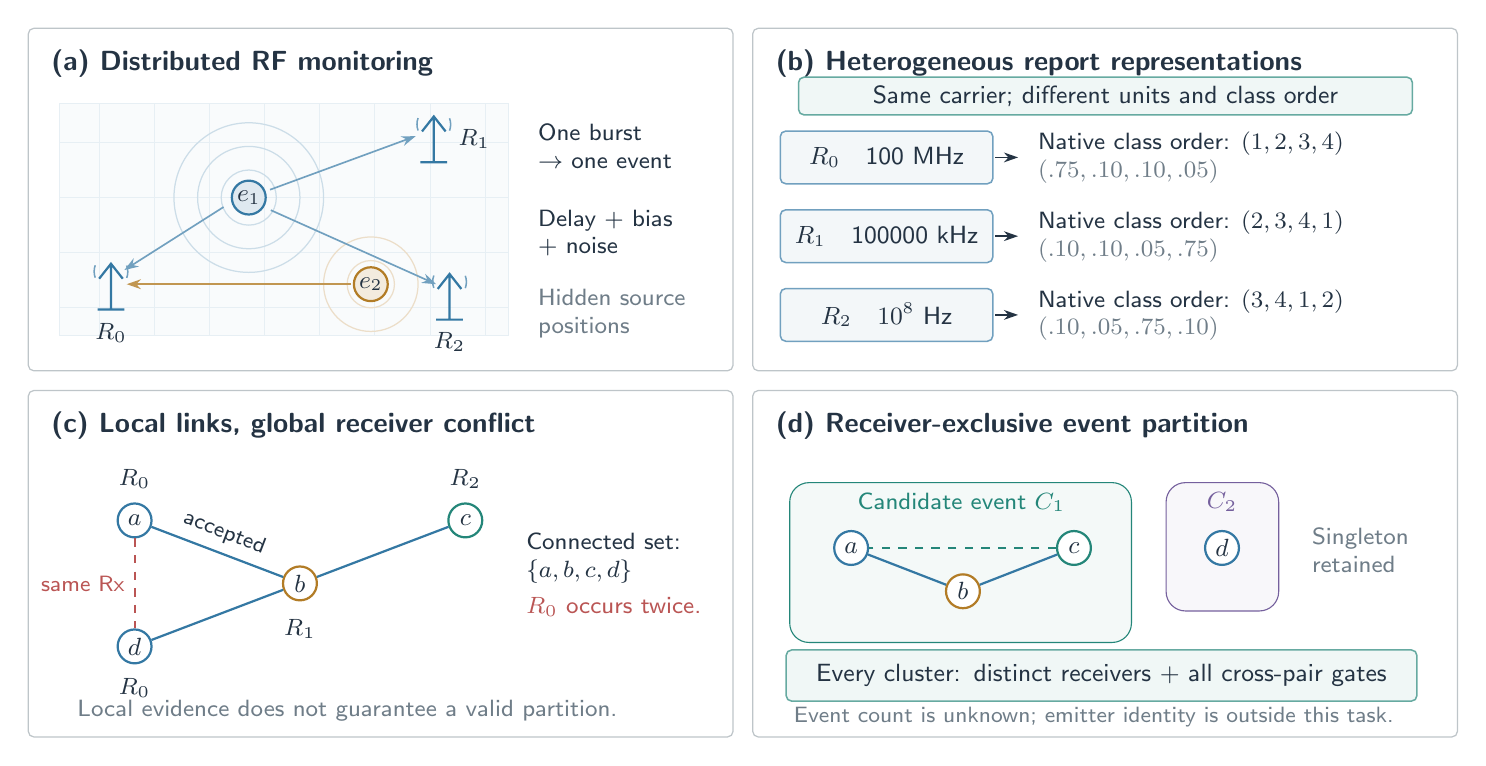
\begin{tikzpicture}[x=1cm,y=1cm]
\draw[panel] (0,4.65) rectangle ++(8.95,4.35);
\node[heading] at (0.17,8.85) {(a) Distributed RF monitoring};
\draw[panel] (9.2,4.65) rectangle ++(8.95,4.35);
\node[heading] at (9.37,8.85) {(b) Heterogeneous report representations};
\draw[panel] (0,0) rectangle ++(8.95,4.4);
\node[heading] at (0.17,4.25) {(c) Local links, global receiver conflict};
\draw[panel] (9.2,0) rectangle ++(8.95,4.4);
\node[heading] at (9.37,4.25) {(d) Receiver-exclusive event partition};

\begin{scope}[shift={(.2,4.75)}]
  \draw[fill=physical!3,draw=physical!12] (.2,.35) rectangle (5.9,3.3);
  \draw[draw=physical!12,step=.7cm,line width=.25pt] (.2,.35) grid (5.9,3.3);
  \coordinate (s1) at (2.6,2.1); \coordinate (s2) at (4.15,1.0);
  \foreach \r in {.35,.65,.95} \draw[physical!25,line width=.45pt] (s1) circle (\r);
  \foreach \r in {.3,.6} \draw[semantic!25,line width=.45pt] (s2) circle (\r);
  \node[dot,fill=physical!16] at (s1) {$e_1$};
  \node[dot,draw=semantic,fill=semantic!15] at (s2) {$e_2$};
  \pic at (.85,.68) {receiver}; \pic at (4.95,2.55) {receiver}; \pic at (5.15,.55) {receiver};
  \node[smalllabel,anchor=north] at (.85,.63) {$R_0$};
  \node[smalllabel,anchor=west] at (5.14,2.85) {$R_1$};
  \node[smalllabel,anchor=north] at (5.15,.51) {$R_2$};
  \draw[edge,physical!70] (2.28,1.98)--(1.02,1.18);
  \draw[edge,physical!70] (2.87,2.20)--(4.72,2.88);
  \draw[edge,physical!70] (2.88,1.94)--(4.98,1.00);
  \draw[edge,semantic!80] (3.9,1.00)--(1.05,1.00);
  \node[align=left,text width=2.1cm,anchor=west,smalllabel] at (6.15,2.75)
    {One burst\\$\rightarrow$ one event};
  \node[align=left,text width=2.1cm,anchor=west,smalllabel] at (6.15,1.65)
    {Delay + bias\\+ noise};
  \node[align=left,text width=2.1cm,anchor=west,smalllabel,text=muted] at (6.15,.63)
    {Hidden source\\positions};
\end{scope}
\begin{scope}[shift={(9.38,4.8)}]
  % Every row is a two-line record.  The top banner ends at y=3.07;
  % all record content starts at y<=2.83 (minimum vertical gap 0.24 cm).
  \node[gate,text width=7.6cm,minimum height=.48cm,inner sep=2.8pt] at (4.3,3.34)
    {Same carrier; different units and class order};
  \foreach \yy/\rx/\val/\ord/\prob in {
     2.56/0/{100 MHz}/{1,2,3,4}/{.75,.10,.10,.05},
     1.56/1/{100000 kHz}/{2,3,4,1}/{.10,.10,.05,.75},
      .56/2/{$10^8$ Hz}/{3,4,1,2}/{.10,.05,.75,.10}
  } {
    \node[box,minimum width=2.70cm,minimum height=.67cm,inner sep=2pt] at (1.52,\yy)
      {\textbf{$R_{\rx}$}\quad \val};
    \draw[edge] (2.90,\yy)--(3.19,\yy);
    \node[smalllabel,anchor=west] at (3.32,\yy+.17)
      {Native class order: $(\ord)$};
    \node[smalllabel,anchor=west,text=muted] at (3.32,\yy-.18)
      {$(\prob)$};
  }
\end{scope}
\begin{scope}[shift={(.35,.3)}]
  \node[dot] (a1) at (1.0,2.45) {$a$};
  \node[dot] (d1) at (1.0,.85) {$d$};
  \node[dot,draw=semantic] (b1) at (3.10,1.65) {$b$};
  \node[dot,draw=feasible] (c1) at (5.2,2.45) {$c$};
  \draw[link] (a1)--node[above,sloped,tinylabel] {accepted} (b1);
  \draw[link] (d1)--(b1); \draw[link] (b1)--(c1);
  \draw[reject] (a1)--node[left,tinylabel,text=fault] {same Rx} (d1);
  \node[smalllabel,anchor=south] at (1,2.73) {$R_0$};
  \node[smalllabel,anchor=north] at (1,.57) {$R_0$};
  \node[smalllabel,anchor=north] at (3.1,1.32) {$R_1$};
  \node[smalllabel,anchor=south] at (5.2,2.73) {$R_2$};
  \node[align=left,text width=2.35cm,anchor=west,smalllabel] at (5.85,1.76)
    {Connected set:\\$\{a,b,c,d\}$\\[3pt]\textcolor{fault}{$R_0$ occurs twice.}};
  \node[smalllabel,text=muted,anchor=west] at (.15,.03) {Local evidence does not guarantee a valid partition.};
\end{scope}
\begin{scope}[shift={(9.45,.3)}]
  \draw[draw=feasible,fill=feasible!5,rounded corners=7pt] (.22,.9) rectangle (4.56,2.93);
  \node[dot] (a2) at (1.0,2.1) {$a$};
  \node[dot,draw=semantic] (b2) at (2.42,1.55) {$b$};
  \node[dot,draw=feasible] (c2) at (3.83,2.1) {$c$};
  \draw[link] (a2)--(b2)--(c2);\draw[draw=feasible,dashed,line width=.8pt] (c2)--(a2);
  \node[smalllabel,text=feasible] at (2.4,2.68) {Candidate event $C_1$};
  \draw[draw=decode,fill=decode!5,rounded corners=7pt] (5.0,1.30) rectangle (6.43,2.93);
  \node[dot] at (5.71,2.1) {$d$};
  \node[smalllabel,text=decode] at (5.71,2.68) {$C_2$};
  \node[smalllabel,text=muted,align=left,anchor=west,text width=1.5cm] at (6.73,2.07)
    {Singleton\\retained};
  \node[gate,text width=7.8cm,minimum height=.65cm] at (4.18,.48)
    {Every cluster: distinct receivers + all cross-pair gates};
  \node[tinylabel,text=muted,anchor=west] at (.15,-.05) {Event count is unknown; emitter identity is outside this task.};
\end{scope}
\end{tikzpicture}
\end{document}
